\documentclass[techrep, submit, noauthor,preface]{ipsj}
%\documentclass{ipsj}
 
\usepackage[dvipdfmx]{graphicx}
\usepackage{amsmath}
\usepackage{amsfonts}
\graphicspath{{./img/}}

\def\Underline{\setbox0\hbox\bgroup\let\\\endUnderline}
\def\endUnderline{\vphantom{y}\egroup\smash{\underline{\box0}}\\}
\def\|{\verb|}

\pagestyle{empty}
\begin{document}

\title{Parameter Unsharingを用いたMode Collapseの回避}

\paffiliate{EI}{慶應義塾大学 環境情報学部}
\paffiliate{GM}{慶應義塾大学 政策メディア研究科}

\author{勝又 海}{}{EI}
\author{小林 凌雅}{}{GM}

\maketitle
\thispagestyle{empty} 
%1
\begin{abstract}

\end{abstract}

\section{序論}

自動運転の研究開発において、virtual evaluationを行うことは非常に重要である。
virtual evaluationではGANを用いてシミュレーション環境をより現実的にしたり、
データセットを拡充したりすることも多い。
しかしGANの研究はまだまだ発展途上であり、学習が不安定であるなどの課題も多い.
そこで我々はGANの安定化の手法としてparameter unsharingを提案した。
GANにはいくつかの問題が存在し、研究開発の発展を妨げている。
1つはGANはGeneratorとDiscriminatorがお互いに競合しあい学習していく手法であり、収束しないことがある。
また、Mode Collapseという現象により、訓練に利用したデータとは似ても似つかない出力をするようになったり、
定数を出力するようになったりする。
これらを回避する手法としてWGANやPacGANなどが提案されている。
Parameter Unsharingでは
学習の際に過去に学習したモデルの重みから遠ざかるように学習させることで別の最適解へ収束させる手法である。
GANのような複雑なモデルの重み空間には多くの局所最適解が存在する.
分類や回帰であればどの局所最適解であってもlossに応じたaccuracyが得られるが, 
GANの場合には同じlossであったとしても全く異なる出力をすることが考えられる.
この手法では別の最適解を探索させることでより良い出力をするモデルを得られる.
また、学習が成功した際にParameter Unsharingを適用させることで異なる表現を得られることを検証した.

\section{関連研究}

{\bf Avoid Mode Collapse on GANs} Mode Collapseを回避する方法としてWGAN, Unrolled GAN, PacGANなどが提案されている.
WGANではWasserstain距離を定義し、Wasserstain距離に基いて学習を行っている。PacGANではミニバッチ中のデータ全てを
1つのデータとして捉えることでデータの分布をより正確に捉えることに成功した.WGANやUnrolled GANは計算コストが高いという
問題点が知られている. またPacGANではDiscriminatorの入力サイズがミニバッチ中の画像を1つの画像として扱うため
Semi Supervised Learningに利用することが出来ない.

{\bf Regularization} ニューラルネットワークの文脈で使われることはそう多くはないが統計学の分野では
Parameter Sharing\cite{deeplearningbook}と呼ばれる手法が使われることがある。
これはモデルを学習させる際に別のモデルの重みに近づくように学習させる手法である。
この手法を反転させた手法を提案した.

\section{手法}

{\bf Generative Adversarial Networks} GeneratorとDiscriminatorを相互に学習させる生成モデルの一種である。
生成モデルとしてはVariational Auto Encoderなど幾つかの手法があるが、鮮明な画像を生成することのできる
生成モデルとしては唯一である。GANの提案後、多くのモデルや応用が研究されており、近年では
自動運転のためのデータセット拡充や、Virtual Evaluationにおいて応用されている.
しかし、学習の不安定さ, Mode Collapse, 定量的な評価が難しいなど多くの課題が残されている. 

{\bf Parameter Unsharing}

通常の目的関数にペナルティ項を加えて目的関数を改良する.

\begin{eqnarray}
  \label{unshare}
  \tilde{\mathcal{L}}(w; X, y, w') =  \frac{\alpha}{2} (w - w')^{\top}(w - w')+ \mathcal{L}(w; X, y)  
\end{eqnarray}


を最適化する。過去のモデルから遠ざけると、もっとも距離が大きくなるのは重みの値が無限大のときである。重みが無限になった場合、lossは大きくなる。これを回避するために重み減衰の項を追加する。


{\bf Parameter Unsharing with MLP}
入力次元が1であるような回帰問題を想定する。入力と出力はそれぞれ
$X = {1, 2, 3, 4, 5,...}$,$y = {4, 16, 36, 64, 100,..}$であり、これを満たす多項式は
$y = (2x)^{2}$もしくは$y = (-2x)^{2}$である。この二つのパラメータを推定させる。

\begin{eqnarray}
  \label{regression}
  \mathcal{L}(w; X, y, w') =  \frac{\alpha}{2} (w - w')^{\top}(w - w') + (f(X) - y)^{2} 
\end{eqnarray}      

と定義する.

{\bf Parameter Unsharing with GANs}

混合正規分布の学習を想定する。目的関数は

\begin{eqnarray}
  \label{gan}
  \mathcal{L}(\theta_{G}, \theta_{D}, \theta'_{G}) & = &  \frac{\alpha}{2} (\theta_{G} - \theta'_{G})^{\top}(\theta_{G} - \theta'_{G})   \nonumber \\
  & & +  \mathbb{E}_{x\sim p_{data}} [ \log(D(x; \theta_{D})) ]   \nonumber \\
  & & + \mathbb{E}_{z\sim \mathcal{N}(0, I)} [ \log(1 - D(G(z;\theta_{G}); \theta_{D})) ]
\end{eqnarray}

と定義する.

\section{実験}

{\bf 多項式フィッテイング}
最適解が複数ある関数の当てはめを行った。今回試したのは$y = ((2or-1)x)^2$である。パーセプトロンを確率的勾配法を用いて最適化を行った。Parameter Unsharingを使わずに最適化を行った場合には重みはランダムに-2もしくは2の値を取った。Parameter Unsharingを用いて最適化を行った場合は遠ざける対象のモデルの重みとは別の符号の値を取った。

{\bf GAN}

平均をずらした正規分布の混合分布から生成させたデータを生成させた. 生成させたの2,3,4つの正規分布の混合分布である。
いずれの場合もParameter Unsharingを繰り返し適用することで目標の分布を捉えることに成功している。

Mode Collapseの回避が可能であることを検証するとともに,
学習がうまくいったと思われるモデルを利用してParameter Unsharingを行った場合の学習結果についても検証を行った。
Unrolled Generative Adversarial Networkを用いて8つの正規分布の混合分布を学習させた。その後、
学習させたモデルを用いてParameter Unsharingによる学習を行った。学習したモデルの出力の散布図を図\ref{fig:unrolled}
に示す.

\begin{figure}[htb]
  \begin{center}
    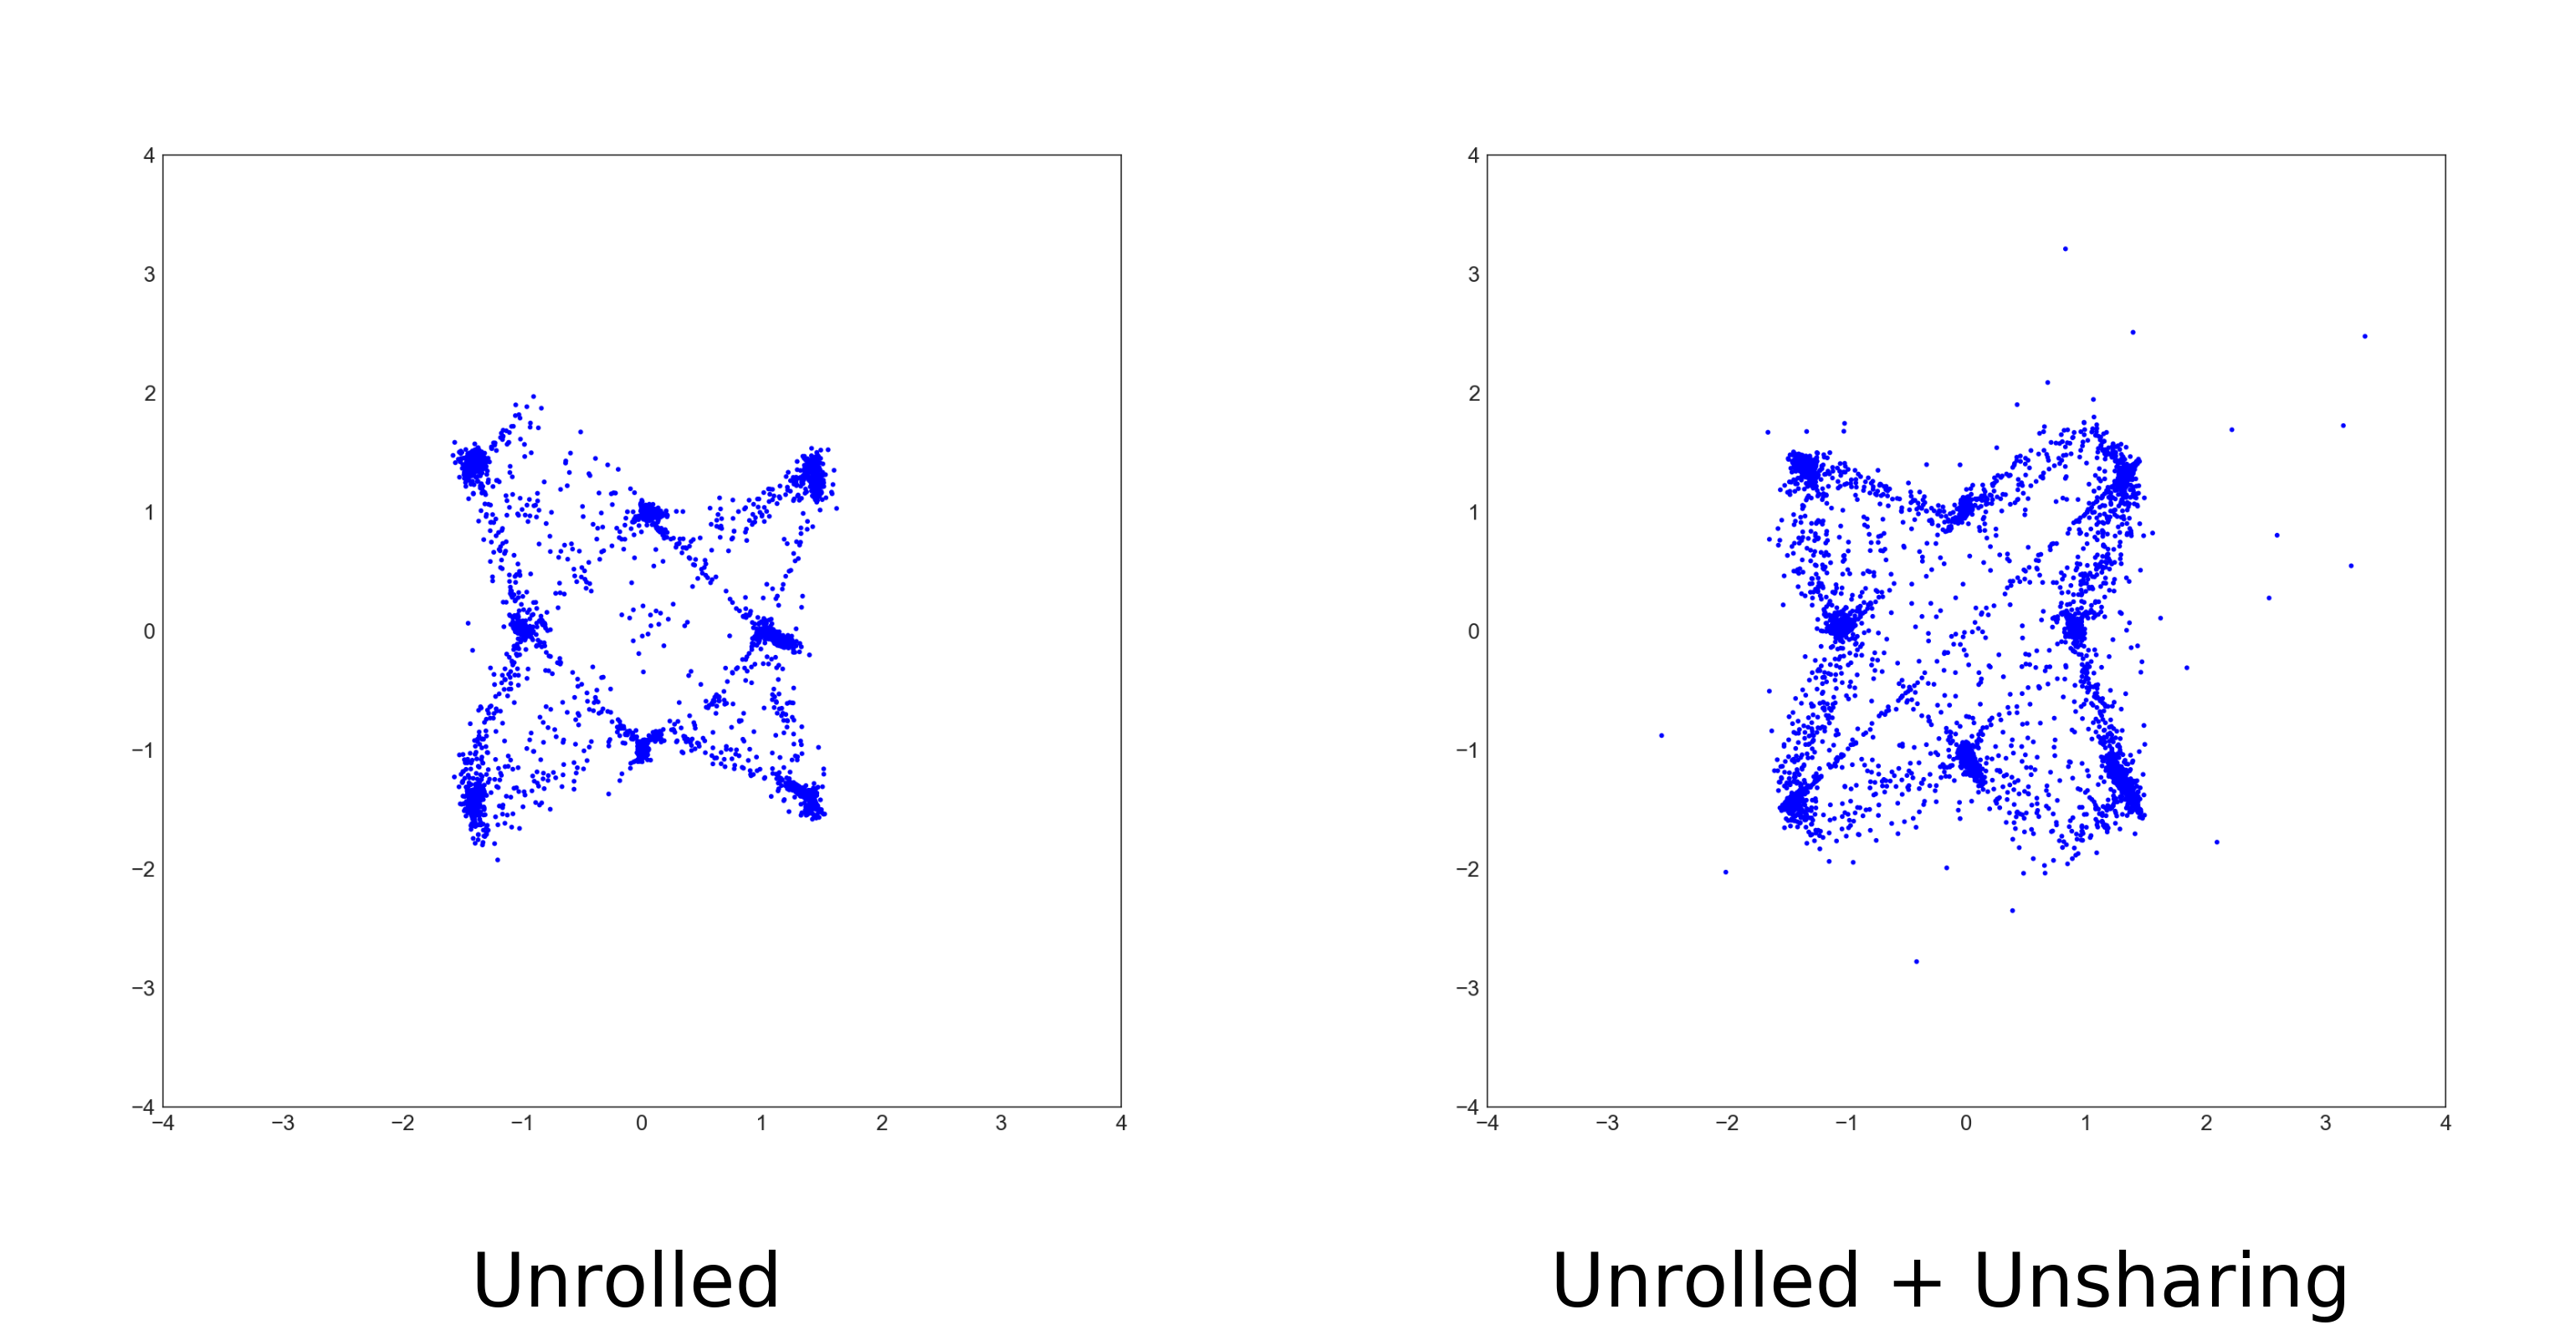
\includegraphics[height=3.5cm]{unrolled.png}
  \end{center}
  \caption{学習したモデルの出力}
  \label{fig:unrolled}
\end{figure}

Prameter Unsharingを行っていても分布を捉えることが出来ている.
また, 元のモデルとは少し異なる表現を獲得していることが分かる.



\section{今後の展望}

我々は提案した手法を用いて異なる最適解の探索が可能であることを検証した。今回、いくつかのモデルに対して適用し、検証を行ったが、他のモデルに対する検証が不十分である。また、学習の安定化に寄与する他の手法との比較が行えていない。他の手法との比較を行うevaluation metricについても研究し、他の手法との比較を行う必要があるo。

\bibliographystyle{ipsjunsrt}
\bibliography{jsample}


\end{document}
